%----------------------------------------------------------------------------------------
%	PACKAGES AND THEMES
%----------------------------------------------------------------------------------------

\documentclass[aspectratio=169,9pt]{beamer}

\mode<presentation> {

  \usetheme{Boadilla} % light

  \usecolortheme{seahorse} % light

  \input{./cvut_colors.tex}

  % \setbeamertemplate{footline} % remove the footer line
  % \setbeamertemplate{footline}[page number] % replace the footer line with simple numbers

  \setbeamertemplate{navigation symbols}{}
  \setbeamertemplate{bibliography item}{\insertbiblabel} % removing the navigation symbols

}

%%{ Docu HEAD

\usepackage{graphicx} % Allows including images
\usepackage{booktabs} % Allows the use of \toprule, \midrule and \bottomrule in tables
\usepackage{multimedia}
\newcommand{\superfill}{\vskip0pt plus 1filll}

\usepackage{isotope}
\usepackage{animate}

\usepackage[export]{adjustbox}

\usepackage{graphicx}
\usepackage{setspace}
\usepackage{epstopdf}
\usepackage{float}
\usepackage{multirow,tabularx,makecell}

\usepackage{pdfpcnotes}

\usefonttheme{professionalfonts}
\usepackage{amsmath,amsfonts,amssymb,bm}

\usepackage[T1]{fontenc}
\usepackage{lmodern}
\usepackage{microtype}

\usepackage[backend=bibtex,defernumbers=true,style=ieee,sorting=none,sortcites=false]{biblatex}

\renewcommand*{\bibfont}{\normalfont\tiny}

% Print labelnumbers with suffixes, adjust secondary labelnumber 2/2
\DeclareFieldFormat{labelnumber}{%
  \ifkeyword{mine}
  {\ifkeyword{core}
  {{\number\numexpr#1}}%
  {{\number\numexpr#1}}%
  }%
  {#1}%
  }

  \DeclareCiteCommand{\tabcite}%[\mkbibbrackets]
  {\usebibmacro{cite:init}%
  \usebibmacro{prenote}}
  {\usebibmacro{citeindex}%
  \usebibmacro{cite:comp}}
  {}
  {\usebibmacro{cite:dump}%
  \usebibmacro{postnote}}

  % {{\number\numexpr#1-\value{bbx:primcount}}a}

  %%{ fullcite box

  \usepackage{tcolorbox}

  \definecolor{light-gray}{gray}{0.95}
  \newcommand{\fullciteinbox}[2]{%

    \DeclareCiteCommand{\fullcite}
    {\usebibmacro{prenote}}
    {\clearfield{addendum}%
    \clearfield{issn}%
    \usedriver
    {\defcounter{minnames}{6}%
    \defcounter{maxnames}{6}}
    {\thefield{entrytype}}}
    {\multicitedelim}
    {\usebibmacro{postnote}}

    %\vspace{3em}%
    %\raisebox{3em}[3em][3em]{%
    % \vspace{-0.2em}
    % \begin{tcolorbox}[width=\textwidth,colback={light-gray},title={}]%
    \begin{block}{}
      \begin{minipage}[t]{0.07\linewidth}%
        \raggedright%
        \scriptsize \cite{#1}%
      \end{minipage}%
      \begin{minipage}[t]{0.93\linewidth}%
        \scriptsize \fullcite{#1}%
        \ifx&#2&
        \else
        \\
        \url{#2}
        \fi
      \end{minipage}%
      % \end{tcolorbox}%
    \end{block}
    %}%
    \vspace{-0.3em}
    }%

    %%}

    \addbibresource{main.bib}

    \defbibenvironment{favoritebib}
  {\itemize}
    {\enditemize}
  {\item}
    \usepackage{siunitx}
    \DeclareSIUnit \parsec {pc}
    \DeclareSIUnit \electronvolt {eV}
    \DeclareSIUnit \pixel {px}
    \DeclareSIUnit \arcmin {arcmin}
    \DeclareSIUnit \erg {erg}
    \DeclareSIUnit \joul {J}
    \DeclareSIUnit \Bq {Bq}

    \usepackage{enumitem} % To enable enumerate with letters (a, b, c...)
    \newlist{alphalist}{enumerate}{1}
    \setlist[alphalist]{label=\alph*)}
    \setlist[itemize]{label=\textbullet}

    \usepackage{cellspace}
    \newcolumntype{D}{>{\hfill}N{3}{2}<{\hfill}}
    \newcommand*\cellspacelimit[2]{\setlength{\cellspacetoplimit}{#1}\setlength{\cellspacebottomlimit}{#2}}

    % figures
    \usepackage{wrapfig}
    % \usepackage[font={footnotesize}]{caption}
    \usepackage[font={small}]{caption}
    % \usepackage{subcaption}

    % subfloat
    \usepackage{subfig}
    % \usepackage[export]{adjustbox}

    \usepackage{color}
    \usepackage{url}

    %%{ tikz

    \usepackage{tikz}
    \usepackage{pgfplots}
    \pgfplotsset{compat=1.14}
    \usetikzlibrary{backgrounds,arrows,automata,shapes,positioning,calc,through,spy,shapes,shapes.geometric,shapes.multipart,fit,patterns,fadings}
    \pgfdeclarelayer{background}
    \pgfdeclarelayer{foreground}
    \pgfsetlayers{background,main,foreground}

    \input{./fig/tikz/tikz.tex}

    \tikzset{
      imgletter/.style={
        rectangle,
        inner sep=2pt,
        rounded corners=.1em,
        text=black,
        minimum height=1em,
        text centered,
        fill=white,
        fill opacity=1.0,
        text opacity=1,
        anchor=south west,
      },
    }

    \input{./tikz-templates_light.tex}

    %%}

    \usepackage{pdfpc-movie}
    \newcommand{\mymovie}[3][]{\pdfpcmovie[#1]{#2}{#3}}
    % \newcommand{\mymovie}[3][]{\movie[#1]{#2}{#3}}

            %%{ CHECKMARK IN TIKZ

            \def\checkmark{\tikz\fill[scale=0.4](0,.35) -- (.25,0) -- (1,.7) -- (.25,.15) -- cycle;}

            %%}

    \newcommand{\strong}[1]{\textbf{#1}}
    \newcommand{\coord}[1]{\textbf{#1}}
    \newcommand{\norm}[1]{\left\lvert#1\right\rvert}
    \newcommand{\m}[1]{\ensuremath{\mathbf{#1}}}
    \newcommand\numberthis{\addtocounter{equation}{1}\tag{\theequation}}
    \newcommand{\corrected}[1]{{\color{black} {#1}}}
    % \newcommand{\comment}[1]{{\color{blue} {#1}}}
    \newcommand{\add}[1]{{\color{green} {#1}}}
    \newcommand{\todo}[1]{{\color{red} TODO {#1}}}
    \newcommand{\updated}[1]{{\color{blue} {#1}}}
    \newcommand{\reffig}[1]{Fig.~\ref{#1}}
    \newcommand{\refalg}[1]{Alg.~\ref{#1}}
    \newcommand{\refsec}[1]{Sec.~\ref{#1}}
    \newcommand{\reftab}[1]{Table~\ref{#1}}
    \newcommand{\real}{\mathbb{R}}
    \newcommand{\red}[1]{{\color{red} #1}}
    \newcommand{\minus}{\scalebox{0.75}[1.0]{$-$}}
    \newcommand{\plus}{\scalebox{0.8}[0.8]{$+$}}
    \newcommand{\figvspace}{\vspace{-1em}} % this may eventually do something, so far just a placeholder

    % \usepackage{pgf}
    % \logo{\pgfputat{\pgfxy(0,5)}{\pgfbox[right,base]{\includegraphics[height=0.8cm]{}}}}
    % \newcommand{\nologo}{\setbeamertemplate{logo}{}}

    % \usepackage{eso-pic}
    % \newcommand\AtPagemyUpperLeft[1]{\AtPageLowerLeft{\put(\LenToUnit{0.66\paperwidth},\LenToUnit{0.904\paperheight}){#1}}}
    % \AddToShipoutPictureFG{
    %   \AtPagemyUpperLeft{{\includegraphics[height=0.85cm,keepaspectratio]{fig/logo_ctu_fee_mrs_blue.png}}}
    % }
    % \newcommand{\AddToShipoutPictureFG}{\setbeamertemplate{logo}{}}

    %%}

\newcommand{\EnvironmentPair}[4]{%
	\makebox[\textwidth][c]{%
		\begin{minipage}[t]{0.49\paperwidth}%
			\begin{figure}%
				\centering%
				\includegraphics[
				width=\linewidth,
				height=0.8\textheight,
				keepaspectratio
				]{#1}%
				\caption{#2}%
			\end{figure}%
		\end{minipage}%
		\hspace{0.005\paperwidth}%
		\begin{minipage}[t]{0.49\paperwidth}%
			\begin{figure}%
				\centering%
				\includegraphics[
				width=\linewidth,
				height=0.8\textheight,
				keepaspectratio
				]{#3}%
				\caption{#4}%
			\end{figure}%
		\end{minipage}%
	}%
}

    %%{ TITLE PAGE


    \title[Bachelor's Thesis]{Rigorous Evaluation of Large-scale
    	Mapping and Localization Systems
    	on High-fidelity Synthetic Datasets}
    \author[Petr Kučera]{{Petr Kučera} \\[0.8em]
    	{\small Supervisor: Ing. David Čapek}
    }
    \institute[FEL CTU in Prague] {
      \begin{small}
        Multi-Robot Systems group, Faculty of Electrical Engineering\\
        Czech Technical University in Prague
      \end{small}}

    \date[June 5th, 2026]{}

    \titlegraphic{\includegraphics[width=5cm]{fig/logo_ctu_fee_mrs_blue.png}}

    \begin{document}

    \begin{frame}

      \titlepage % Print the title page as the first slide

    \end{frame}

    % \nologo

    %%}

\begin{frame}
\frametitle{Problem Introduction}

\begin{columns}[T,onlytextwidth]
	
\begin{column}{0.35\textwidth}
	\begin{itemize}
	\item Opportunities to evaluate UAV systems in challenging real-world environments are limited.
	\item High-fidelity virtual environments are needed for simulation, testing and training.
	\item Manual creation of realistic virtual environments is challenging and time consuming process.
	\end{itemize}
\end{column}
\begin{column}{0.65\textwidth}
	\begin{figure}[h]
		\centering%
		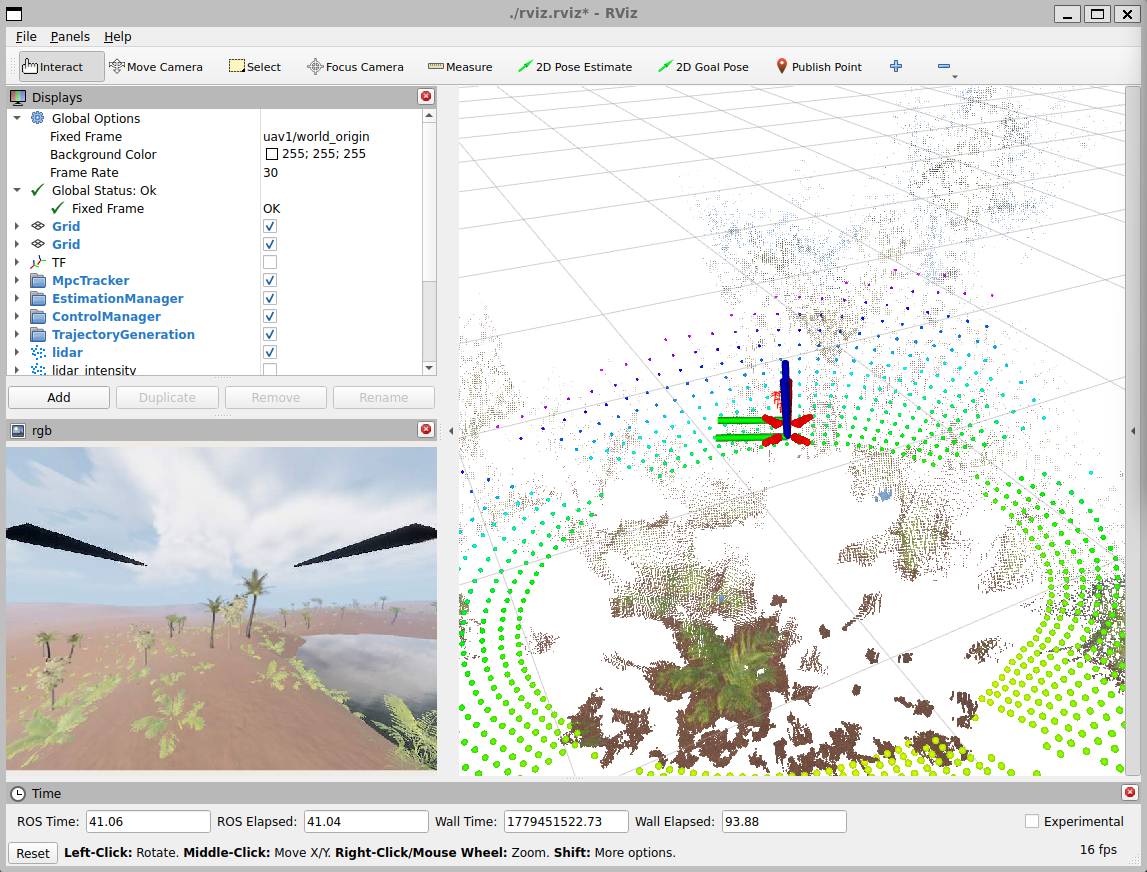
\includegraphics[keepaspectratio,height=7cm]{fig/screenshots/simulation.png}
	\end{figure}
\end{column}
	
\end{columns}

\end{frame}

\begin{frame}
\frametitle{Thesis Objectives}

% todo obrázek here asi taky ale jaký??? Nebo udělat 2/3 blocky vedle sebe?

\begin{columns}[T,onlytextwidth]

\begin{column}{0.45\textwidth}
	\begin{itemize}
		\item Design a method of autonomous environment generation.
		\item Implement the workflow as an Unreal Engine~5 plugin.
		\item Generate multiple environments using the proposed method.
		\item Create datasets from the generated environments using the Flight Forge simulator.
		\item Evaluate selected mapping frameworks using the created datasets.
	\end{itemize}
\end{column}

\end{columns}

\end{frame}

\begin{frame}
\frametitle{Proposed Pipeline}

\begin{figure}
	\begin{adjustbox}{max totalsize={1.1\textwidth}{.75\textheight}, center}
		\pgfdeclarelayer{foreground}
\pgfsetlayers{background,main,foreground}

\tikzset{radiation/.style={{decorate,decoration={expanding waves,angle=90,segment length=4pt}}}}

\begin{tikzpicture}[->,>=stealth', node distance=3.0cm,scale=1.0, every node/.style={scale=1.0}]

	\node[state, shift = {(0.0, 6.0)}] (in_hm) {
	 	\begin{tabular}{c}
	 		\footnotesize Provided\\
	 		\footnotesize height map\\
	 		\footnotesize (Grayscale Image)
	 	\end{tabular}
	};
	
	\node[state, shift = {(0.0, 3.0)}] (in_si) {
	 	\begin{tabular}{c}
	 		\footnotesize Provided\\
	 		\footnotesize segmentation\\
	 		\footnotesize (RGB Image)
	 	\end{tabular}
	};
	
	\node[state, shift = {(0.0, 0.0)}] (in_sl) {
	 	\begin{tabular}{c}
	 		\footnotesize Provided\\
	 		\footnotesize segmentation legend\\
	 		\footnotesize (JSON file)
	 	\end{tabular}
	};
	
	\node[state, shift = {(5.0, 6.0)}] (ls_gen) {
	 	\begin{tabular}{c}
	 		\footnotesize Landsapce\\
	 		\footnotesize Generation
	 	\end{tabular}
	};
	
	\node[state, shift = {(5.0, 3.0)}] (bm_ex) {
	 	\begin{tabular}{c}
	 		\footnotesize Binary Mask\\
	 		\footnotesize Creation
	 	\end{tabular}
	};
	
	\node[state, shift = {(10.0, 5.0)}] (bm_skel) {
		\begin{tabular}{c}
			\footnotesize Binary Mask\\
			\footnotesize Skeletonization
		\end{tabular}
	};
	
	\node[state, shift = {(10.0, 1.0)}] (bm_con) {
		\begin{tabular}{c}
			\footnotesize Binary Mask\\
			\footnotesize Contours
		\end{tabular}
	};
	
	\node[state, shift = {(15.0, 4.0)}] (rs) {
		\begin{tabular}{c}
			\footnotesize River Splines
		\end{tabular}
	};
	
	\node[state, shift = {(15.0, 6.0)}] (ls) {
		\begin{tabular}{c}
			\footnotesize Landscape Splines\\
			\footnotesize (Roads)
		\end{tabular}
	};
	
	\node[state, shift = {(15.0, 2.0)}] (ws) {
		\begin{tabular}{c}
			\footnotesize Lake Splines
		\end{tabular}
	};
	
	\node[state, shift = {(15.0, 0.0)}] (bs) {
		\begin{tabular}{c}
			\footnotesize Biome Region\\
			\footnotesize Splines
		\end{tabular}
	};
  
  
	\path[->] ($(in_hm.east) + (0.0, 0)$) edge [] node[above, midway, shift = {(0.0, 0.05)}] {
	  	\begin{tabular}{c}
	  		\footnotesize Height map is\\
	  		\footnotesize upscaled to the\\
	  		\footnotesize user preference
	\end{tabular}} ($(ls_gen.west) + (0.0, 0.00)$);

	\path[->] ($(in_si.east) + (0.0, 0)$) edge [] node[above, midway, shift = {(1.0, -1.95)}] {
		\begin{tabular}{c}
			\footnotesize Segmentation Legend is\\
			\footnotesize used to create binary\\
			\footnotesize mask from segmentation
	\end{tabular}} ($(bm_ex.west) + (0.0, 0.00)$);

	\path[-] ($(in_sl.east) + (0.0, 0)$) edge [] node[above, midway, shift = {(0.0, 0.0)}] {}
	($(in_sl.east -| bm_ex.south)$) -- ($(in_sl.east -| bm_ex.south)$)
	edge [->] ($(bm_ex.south)+(0, 0)$);
  
	\path[-] ($(bm_ex.east) + (0.0, 0)$) edge [] node[above, midway, shift = {(3.25, -0.9)}] {
		\begin{tabular}{c}
			\footnotesize Splines are\\
			\footnotesize interpolated from\\
			\footnotesize extracted skeletons\\
			\footnotesize and contours.
		\end{tabular}}
	($(bm_ex.center) + (2.5, 0)$) -- ($(bm_ex.center) + (2.5, 0)$)
	edge [] ($(bm_ex.center) + (2.5, -2)$) -- ($(bm_ex.center) + (2.5, -2)$) edge [->] ($(bm_con.west) + (0.0, 0)$);
	
	\path[-] ($(bm_ex.east) + (0.0, 0)$) edge [] node[above, midway, shift = {(0.0, 0.0)}] {}
	($(bm_ex.center) + (2.5, 0)$) -- ($(bm_ex.center) + (2.5, 0)$)
	edge [] ($(bm_ex.center) + (2.5, 2)$) -- ($(bm_ex.center) + (2.5, 2)$) edge [->] ($(bm_skel.west) + (0.0, 0)$);
	
	\path[-] ($(bm_skel.east) + (0.0, 0)$) edge [] node[above, midway, shift = {(0.0, 0.0)}] {}
	($(bm_skel.center) + (2.5, 0)$) -- ($(bm_skel.center) + (2.5, 0)$)
	edge [] ($(bm_skel.center) + (2.5, 1)$) -- ($(bm_skel.center) + (2.5, 1)$) edge [->] ($(ls.west) + (0.0, 0)$);
	
	\path[-] ($(bm_skel.east) + (0.0, 0)$) edge [] node[above, midway, shift = {(0.0, 0.0)}] {}
	($(bm_skel.center) + (2.5, 0)$) -- ($(bm_skel.center) + (2.5, 0)$)
	edge [] ($(bm_skel.center) + (2.5, -1)$) -- ($(bm_skel.center) + (2.5, -1)$) edge [->] ($(rs.west) + (0.0, 0)$);
	
	\path[-] ($(bm_con.east) + (0.0, 0)$) edge [] node[above, midway, shift = {(0.0, 0.0)}] {}
	($(bm_con.center) + (2.5, 0)$) -- ($(bm_con.center) + (2.5, 0)$)
	edge [] ($(bm_con.center) + (2.5, 1)$) -- ($(bm_con.center) + (2.5, 1)$) edge [->] ($(ws.west) + (0.0, 0)$);
	
	\path[-] ($(bm_con.east) + (0.0, 0)$) edge [] node[above, midway, shift = {(0.0, 0.0)}] {}
	($(bm_con.center) + (2.5, 0)$) -- ($(bm_con.center) + (2.5, 0)$)
	edge [] ($(bm_con.center) + (2.5, -1)$) -- ($(bm_con.center) + (2.5, -1)$) edge [->] ($(bs.west) + (0.0, 0)$);
	
	\path[dashed,<-] ($(ls_gen.east) + (0.0, 0)$) edge [] node[above, midway, shift = {(0.0, 0.05)}] {\begin{tabular}{c}
			\footnotesize Modifies and deforms \\
			\footnotesize generated landspace
	\end{tabular}}
	($(bm_skel.east) + (0.8, 1)$) -- ($(bm_skel.east) + (0.8, 1)$)
	edge [-] ($(bm_skel.east) + (0.8, 1.2)$) -- ($(bm_skel.east) + (0.8, 1.2)$) edge [-] ($(ls.west) + (0.0, 0.2)$);
	
	\path[dashed,<-] ($(ls_gen.east) + (0.0, 0)$) edge [] node[above, midway, shift = {(0.0, 0.0)}] {}
	($(bm_skel.east) + (0.8, 1)$) -- ($(bm_skel.east) + (0.8, 1)$)
	edge [-] ($(bm_skel.east) + (0.8, -0.8)$) -- ($(bm_skel.east) + (0.8, -0.8)$) edge [-] ($(rs.west) + (0.0, 0.2)$);
	
	\path[dashed,<-] ($(ls_gen.east) + (0.0, 0)$) edge [] node[above, midway, shift = {(0.0, 0.0)}] {}
	($(bm_skel.east) + (0.8, 1)$) -- ($(bm_skel.east) + (0.8, 1)$)
	edge [-] ($(bm_skel.east) + (0.8, -2.8)$) -- ($(bm_skel.east) + (0.8, -2.8)$) edge [-] ($(ws.west) + (0.0, 0.2)$);
	
	\path[dashed,<-] ($(ls_gen.east) + (0.0, 0)$) edge [] node[above, midway, shift = {(0.0, 0.0)}] {}
	($(bm_skel.east) + (0.8, 1)$) -- ($(bm_skel.east) + (0.8, 1)$)
	edge [-] ($(bm_skel.east) + (0.8, -4.8)$) -- ($(bm_skel.east) + (0.8, -4.8)$) edge [-] ($(bs.west) + (0.0, 0.2)$);
\end{tikzpicture}


	\end{adjustbox}
\end{figure}

\end{frame}

\begin{frame}
\frametitle{Binary Mask Skeletonization}	

\begin{columns}[T,onlytextwidth]

\begin{column}{0.45\textwidth}
	\begin{block}{Skeletonization}
		\begin{itemize}
			\item Jain--Kumar thinning algorithm.
			\item Creates a 1-pixel-wide skeleton from a binary mask.
			\item May create undesired branches if the mask does not have smooth outlines.
			\item The 1-pixel-wide skeleton simplifies polyline extraction and spline interpolation.
		\end{itemize}
	\end{block}	
	
	\begin{block}{Mask Smoothing}
		\begin{itemize}
			\item Smoothing is performed using a Gaussian blur.
			\item Reduces undesired branching of the skeleton while maintaining the general shape of the skeleton.
		\end{itemize}
	\end{block}	
\end{column}

\begin{column}{0.45\textwidth}
	\begin{figure}[h]
		\centering%
		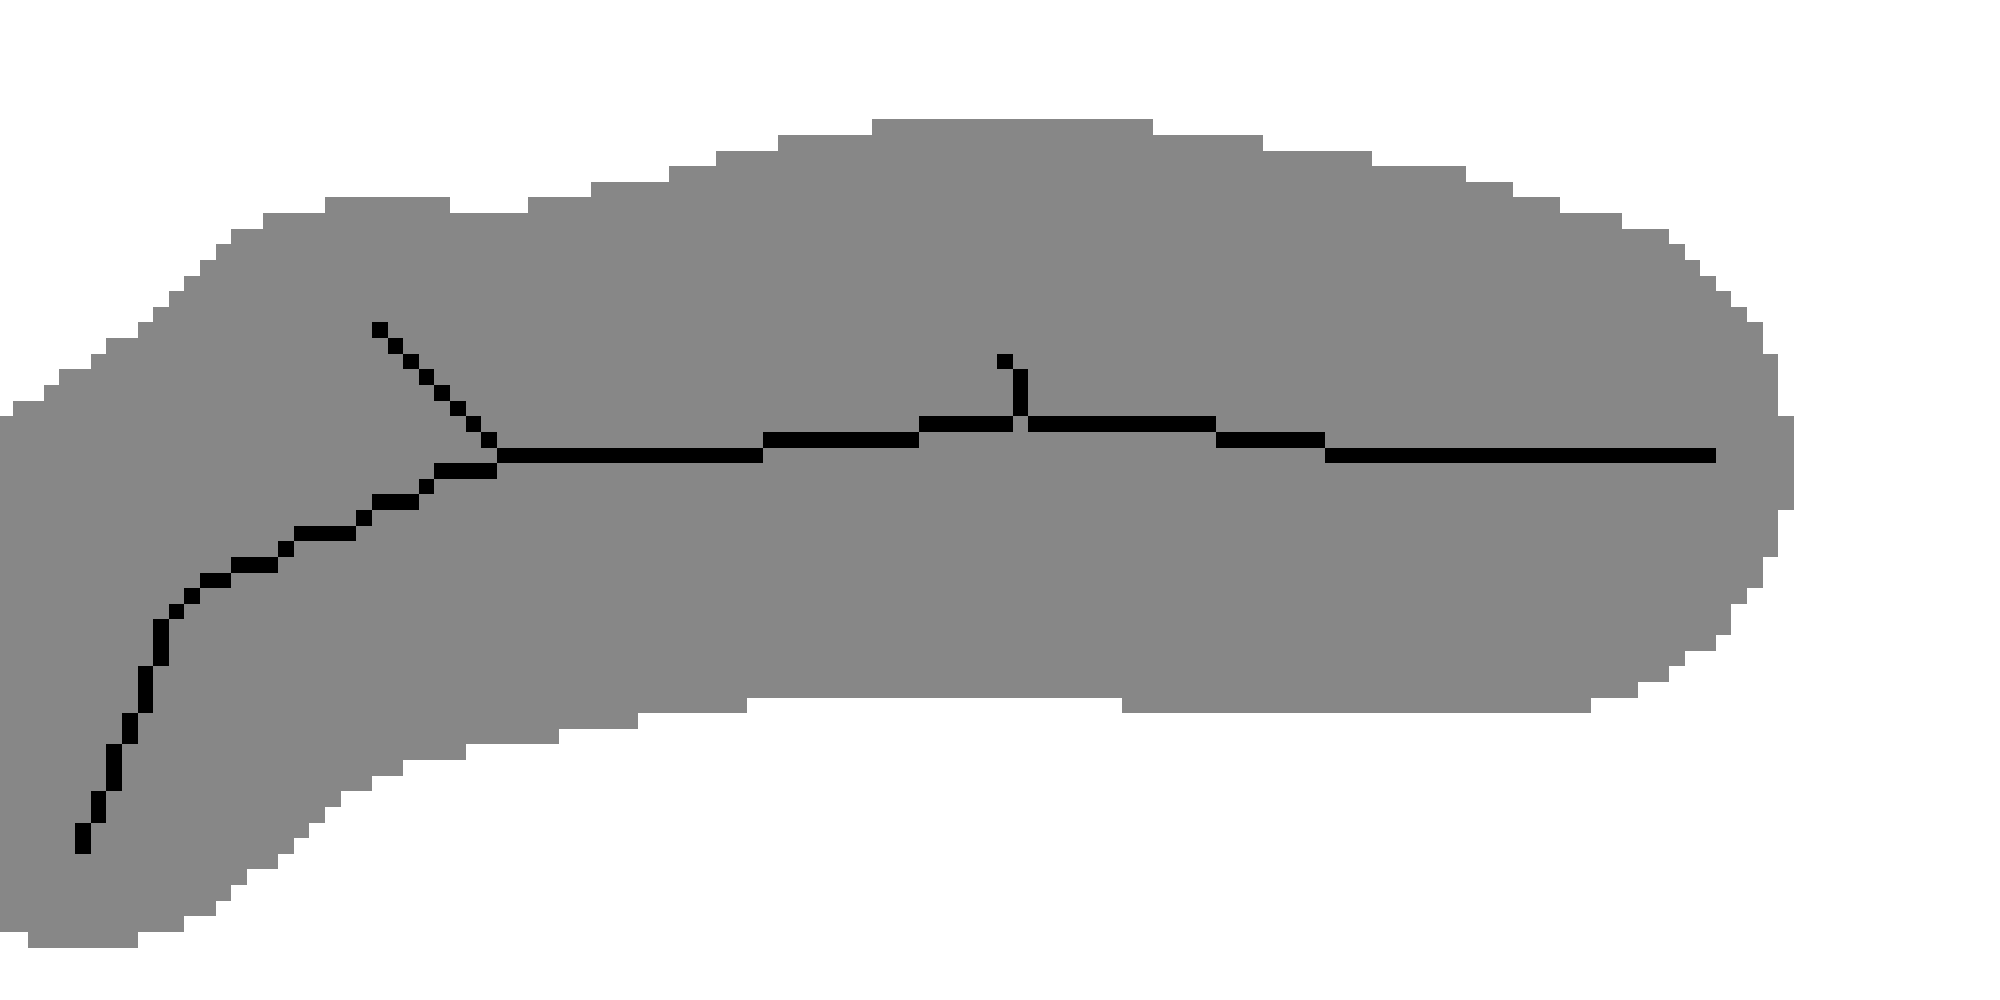
\includegraphics[keepaspectratio,height=2.5cm]{fig/screenshots/image_skel_1.png}
		\caption{Skeletonization without mask smoothing}
	\end{figure}
	
	\begin{figure}[h]
		\centering%
		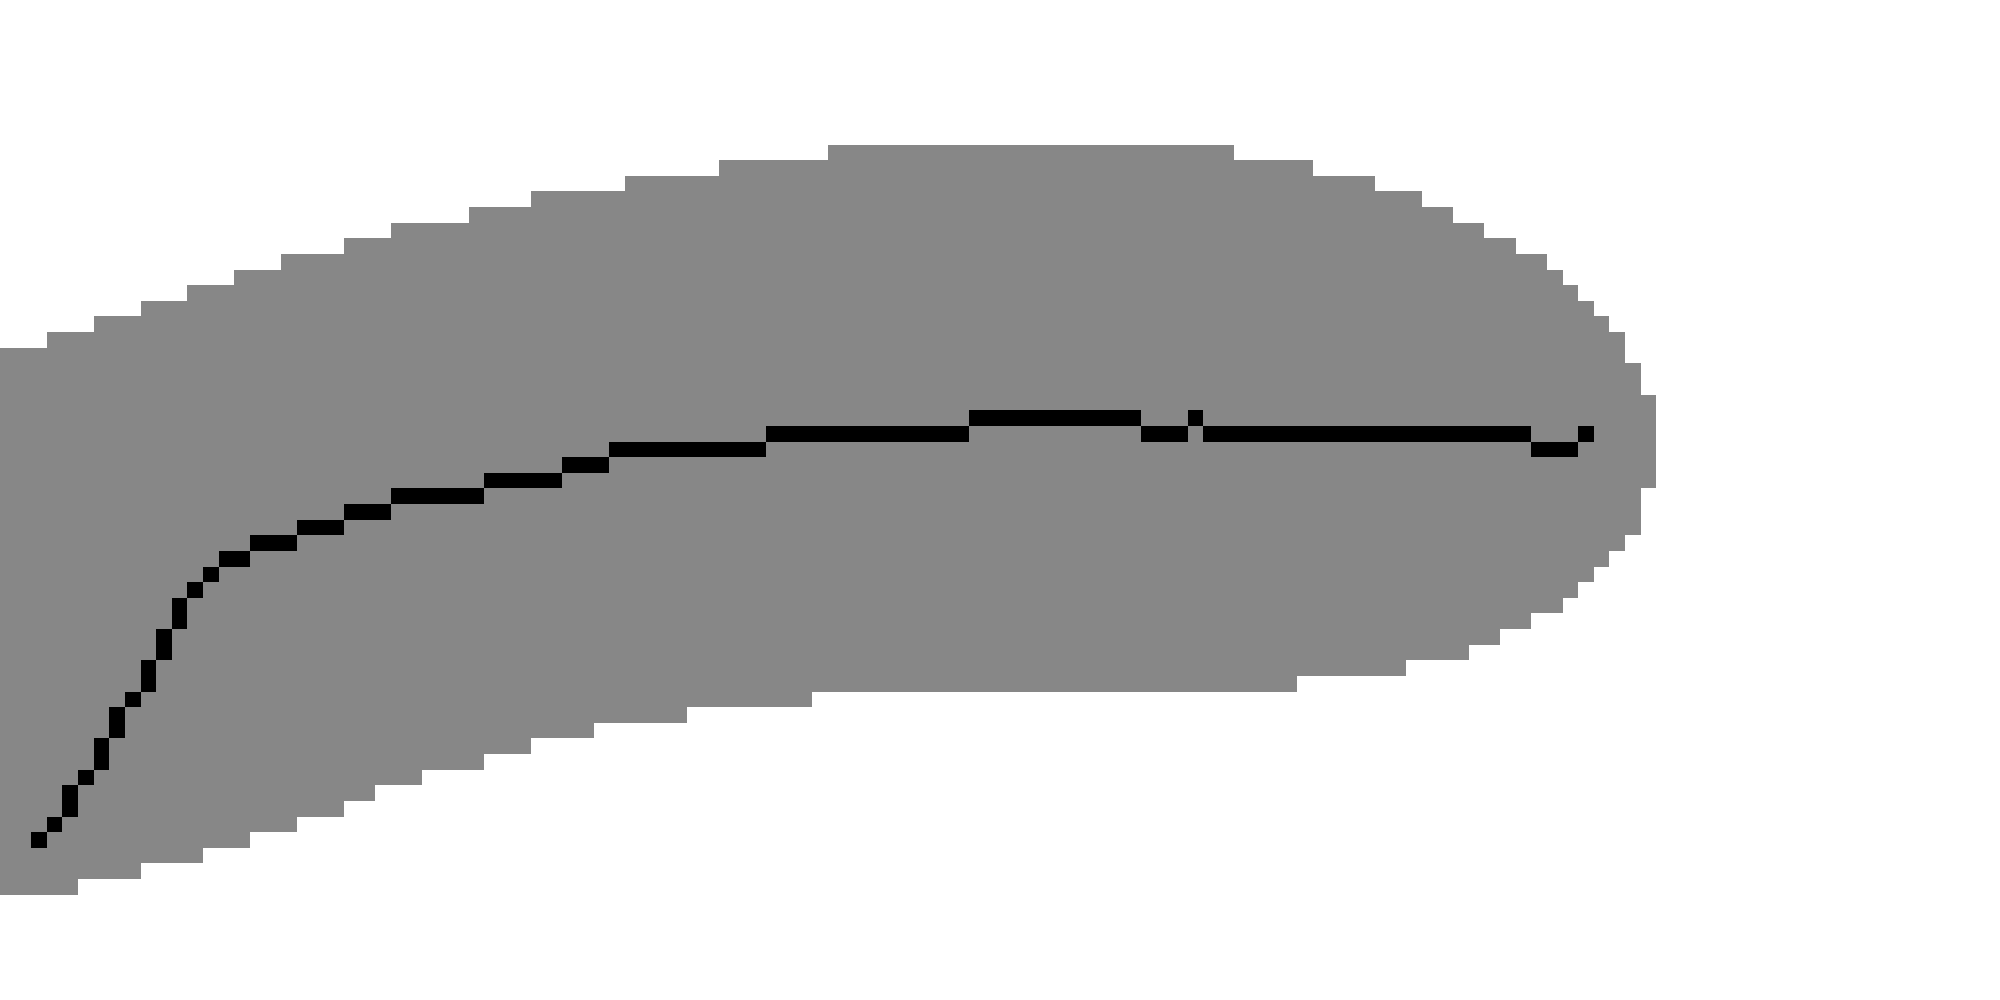
\includegraphics[keepaspectratio,height=2.5cm]{fig/screenshots/image_skel_2.png}%
		\caption{Skeletonization with mask smoothing}
	\end{figure}
\end{column}

\end{columns}

\end{frame}

\begin{frame}
\frametitle{Biome Representation}

\vspace*{-0.4cm}

\begin{columns}[T,onlytextwidth]
	
\begin{column}{0.45\textwidth}
	\begin{block}{Biome Map}
		\begin{itemize}
			\item Segmentation image can be used directly as a biome map.
			\item Faster biome creation.
			\item Difficult to adjust manually.
		\end{itemize}
	\end{block}
	
	\begin{figure}[h]
		\centering%
		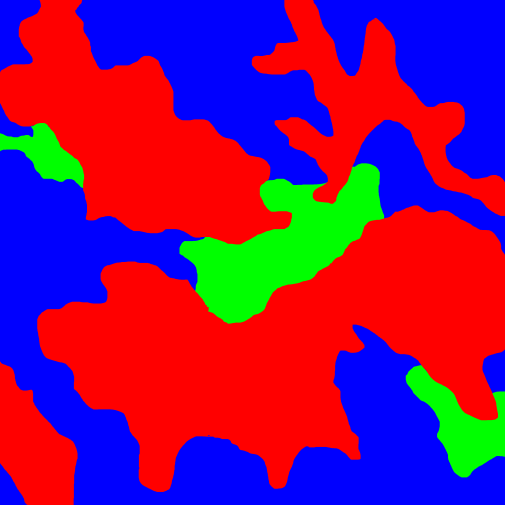
\includegraphics[keepaspectratio,height=5cm]{fig/screenshots/biome_map.png}
	\end{figure}
	
\end{column}

\begin{column}{0.45\textwidth}
	\begin{block}{Biome Spline}
		\begin{itemize}
			\item Biome boundaries are represented by editable splines.
			\item Easier manual adjustment.
			\item More time-consuming to create and configure.
		\end{itemize}
	\end{block}
	
	\begin{figure}[h]
		\centering%
		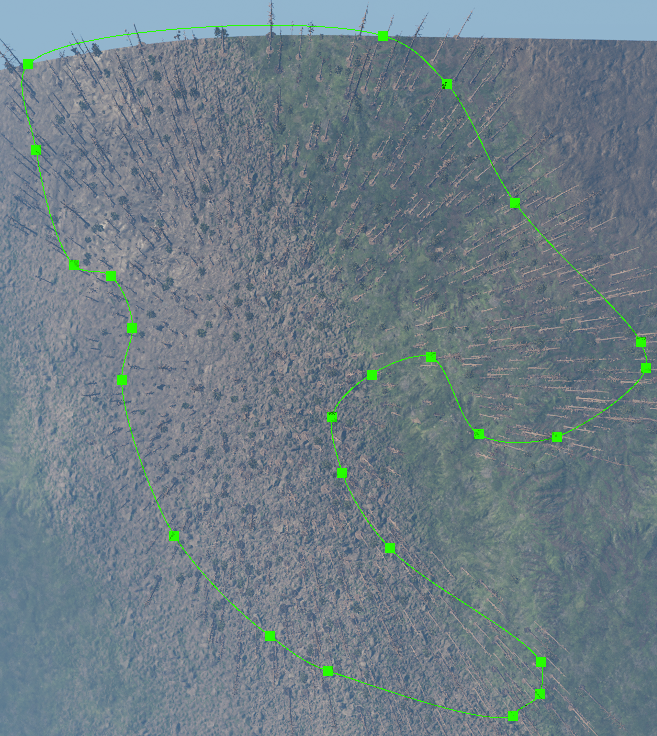
\includegraphics[keepaspectratio,height=5cm]{fig/screenshots/biome_spline.png}
	\end{figure}
\end{column}
	
\end{columns}
	
\end{frame}

% \begin{frame}[t]
% \frametitle{Polyline Point Reduction}	
	
% \begin{columns}[T,onlytextwidth]

% \begin{column}{0.60\textwidth}
% 	\begin{figure}
% 		\hspace*{-1cm}
% 		\begin{adjustbox}{scale=1.5, center}
% 			% douglas_peucker.tex
% Requires in main preamble:
% \usepackage{tikz}

% Original polyline path - for plot coordinates, NO commas between coordinates
\def\RawPath{
	(0,0) (1,1) (2,2) (2,3) (3,4) (4,5) (4,6) (5,7) (5,8) (6,9)
	(7,10) (7,11) (8,12) (8,13) (9,14) (9,15) (10,16) (11,17) (12,18) (13,18)
	(14,19) (15,19) (16,19) (17,20) (18,20) (19,20) (20,21) (21,21) (22,21) (23,22)
	(24,22) (25,22) (26,22) (27,22) (28,22) (29,23) (30,23) (31,23) (32,23) (33,23)
	(34,24) (35,24) (36,24) (37,25) (38,25) (39,25) (40,25) (41,25) (42,25) (43,25)
	(44,25) (45,25) (46,25) (47,26) (48,26) (49,26) (50,26) (51,26) (52,26) (53,26)
	(54,26) (55,26) (56,26) (57,26) (58,26) (59,26) (60,27) (61,27) (62,27) (63,27)
	(64,27) (65,27) (66,27) (67,27) (68,27) (69,27) (70,27) (71,26) (72,26) (73,26)
	(74,27) (75,26) (76,26) (77,26) (78,26) (79,26) (80,26) (81,26) (82,26) (83,26)
	(84,26) (85,26) (86,26) (87,26) (88,26) (89,26) (90,26) (91,26) (92,26) (93,26)
	(94,26) (95,26) (96,25) (97,25) (98,25) (99,26)
}

% Original polyline list - for foreach, coordinates must be wrapped in braces
\def\RawList{
	{(0,0)},{(1,1)},{(2,2)},{(2,3)},{(3,4)},{(4,5)},{(4,6)},{(5,7)},{(5,8)},{(6,9)},
	{(7,10)},{(7,11)},{(8,12)},{(8,13)},{(9,14)},{(9,15)},{(10,16)},{(11,17)},{(12,18)},{(13,18)},
	{(14,19)},{(15,19)},{(16,19)},{(17,20)},{(18,20)},{(19,20)},{(20,21)},{(21,21)},{(22,21)},{(23,22)},
	{(24,22)},{(25,22)},{(26,22)},{(27,22)},{(28,22)},{(29,23)},{(30,23)},{(31,23)},{(32,23)},{(33,23)},
	{(34,24)},{(35,24)},{(36,24)},{(37,25)},{(38,25)},{(39,25)},{(40,25)},{(41,25)},{(42,25)},{(43,25)},
	{(44,25)},{(45,25)},{(46,25)},{(47,26)},{(48,26)},{(49,26)},{(50,26)},{(51,26)},{(52,26)},{(53,26)},
	{(54,26)},{(55,26)},{(56,26)},{(57,26)},{(58,26)},{(59,26)},{(60,27)},{(61,27)},{(62,27)},{(63,27)},
	{(64,27)},{(65,27)},{(66,27)},{(67,27)},{(68,27)},{(69,27)},{(70,27)},{(71,26)},{(72,26)},{(73,26)},
	{(74,27)},{(75,26)},{(76,26)},{(77,26)},{(78,26)},{(79,26)},{(80,26)},{(81,26)},{(82,26)},{(83,26)},
	{(84,26)},{(85,26)},{(86,26)},{(87,26)},{(88,26)},{(89,26)},{(90,26)},{(91,26)},{(92,26)},{(93,26)},
	{(94,26)},{(95,26)},{(96,25)},{(97,25)},{(98,25)},{(99,26)}
}

% Douglas-Peucker result
\def\DpPath{
	(0,0) (12,18) (23,22) (60,27) (99,26)
}

\def\DpList{
	{(0,0)},{(12,18)},{(23,22)},{(60,27)},{(99,26)}
}

\begin{tikzpicture}[
	x=0.055cm,
	y=0.055cm,
	line cap=round,
	line join=round
	]
	
	% =========================================================
	% Original polyline
	% =========================================================
	\begin{scope}[shift={(0,38)}]
		\node[anchor=west, font=\scriptsize] at (0,32) {Original polyline: 106 points};
		
		\draw[black, line width=0.5pt] plot coordinates {\RawPath};
		
		\foreach \p in \RawList {
			\fill[red] \p circle (1.0pt);
		}
	\end{scope}
	
	% =========================================================
	% Douglas-Peucker simplified polyline
	% =========================================================
	\begin{scope}[shift={(0,-6)}]
		\node[anchor=west, font=\scriptsize] at (0,32) {Douglas--Peucker reduction: 5 points};
		
		% Original in background
		\draw[gray!55, line width=0.35pt] plot coordinates {\RawPath};
		
		\foreach \p in \RawList {
			\fill[gray!55] \p circle (0.45pt);
		}
		
		% Simplified result
		\draw[blue, line width=1.1pt] plot coordinates {\DpPath};
		
		\foreach \p in \DpList {
			\fill[red] \p circle (1.35pt);
		}
	\end{scope}
	
\end{tikzpicture}
% 		\end{adjustbox}
% 	\end{figure}
% \end{column}

% \begin{column}{0.40\textwidth}
% 	\begin{block}{Polyline Point Reduction}
% 		\begin{itemize}
% 			\item Polylines created from skeletons may contain large amount of redundant points.
% 			\item Douglas--Peucker Algorithm.
% 			\item The amount of points is reduced while maintaining the general shape of the polyline.
% 		\end{itemize}
% 	\end{block}
% \end{column}

% \end{columns}
	
% \end{frame}

% \begin{frame}[t]
% \frametitle{Spline Interpolation}	

% \begin{tikzpicture}[remember picture,overlay]
% 	\node[
% 	anchor=south east,
% 	inner sep=0pt
% 	] at ([xshift=-1cm,yshift=-0.5cm]current page.south east) {%
% 		\includegraphics[
% 		keepaspectratio,
% 		height=6.4cm
% 		]{fig/pdf/catmull_rom.pdf}%
% 	};
% \end{tikzpicture}

% \vspace*{-0.7cm}

% \begin{columns}[T,onlytextwidth]

% \begin{column}{0.45\textwidth}
% 	\begin{block}{Spline Interpolation}
% 		\begin{itemize}
% 			\item Catmull--Rom Spline Interpolation from polyline algorithm creates B\'ezier curves.
% 			\item B\'ezier curves are easily converted to Hermite splines, which are used by Unreal Engine~5.
% 			\item B\'ezier curves can be subdivided using de Casteljau's algorithm.
% 		\end{itemize}
% 	\end{block}
% \end{column}

% \begin{column}{0.45\textwidth}
% 	% Empty column, image is drawn in background
% \end{column}

% \end{columns}
	
% \end{frame}

\begin{frame}[t]
\frametitle{Generated Environments}

\vspace*{-0.1cm}

\EnvironmentPair
{fig/screenshots/desert_oasis_1.jpg}
{Desert Oasis}
{fig/screenshots/etretat_cliffs_1.jpg}
{\'{E}tretat Cliffs}

\end{frame}

\begin{frame}[t]
\frametitle{Generated Environments}

\vspace*{-0.1cm}

\EnvironmentPair
{fig/screenshots/grand_canyon_2.jpg}
{Grand Canyon}
{fig/screenshots/studlagil_canyon_1.jpg}
{Stu{\dh}lagil Canyon}

\end{frame}

\begin{frame}[t]
\frametitle{Performance Metrics}	

\vspace*{-0.5cm}

\begin{columns}[T,onlytextwidth]

\begin{column}{0.38\textwidth}
	\vspace*{1cm}
	\begin{block}{Datasets and Verification}
		\begin{itemize}
			\item 10 datasets were created on the generated environments.
			\item Captured performance metrics: CPU Usage, Memory Usage and Point cloud insertion time.
		\end{itemize}
	\end{block}
\end{column}

\begin{column}{0.6\textwidth}
	\begin{figure}[h]
		\centering%
		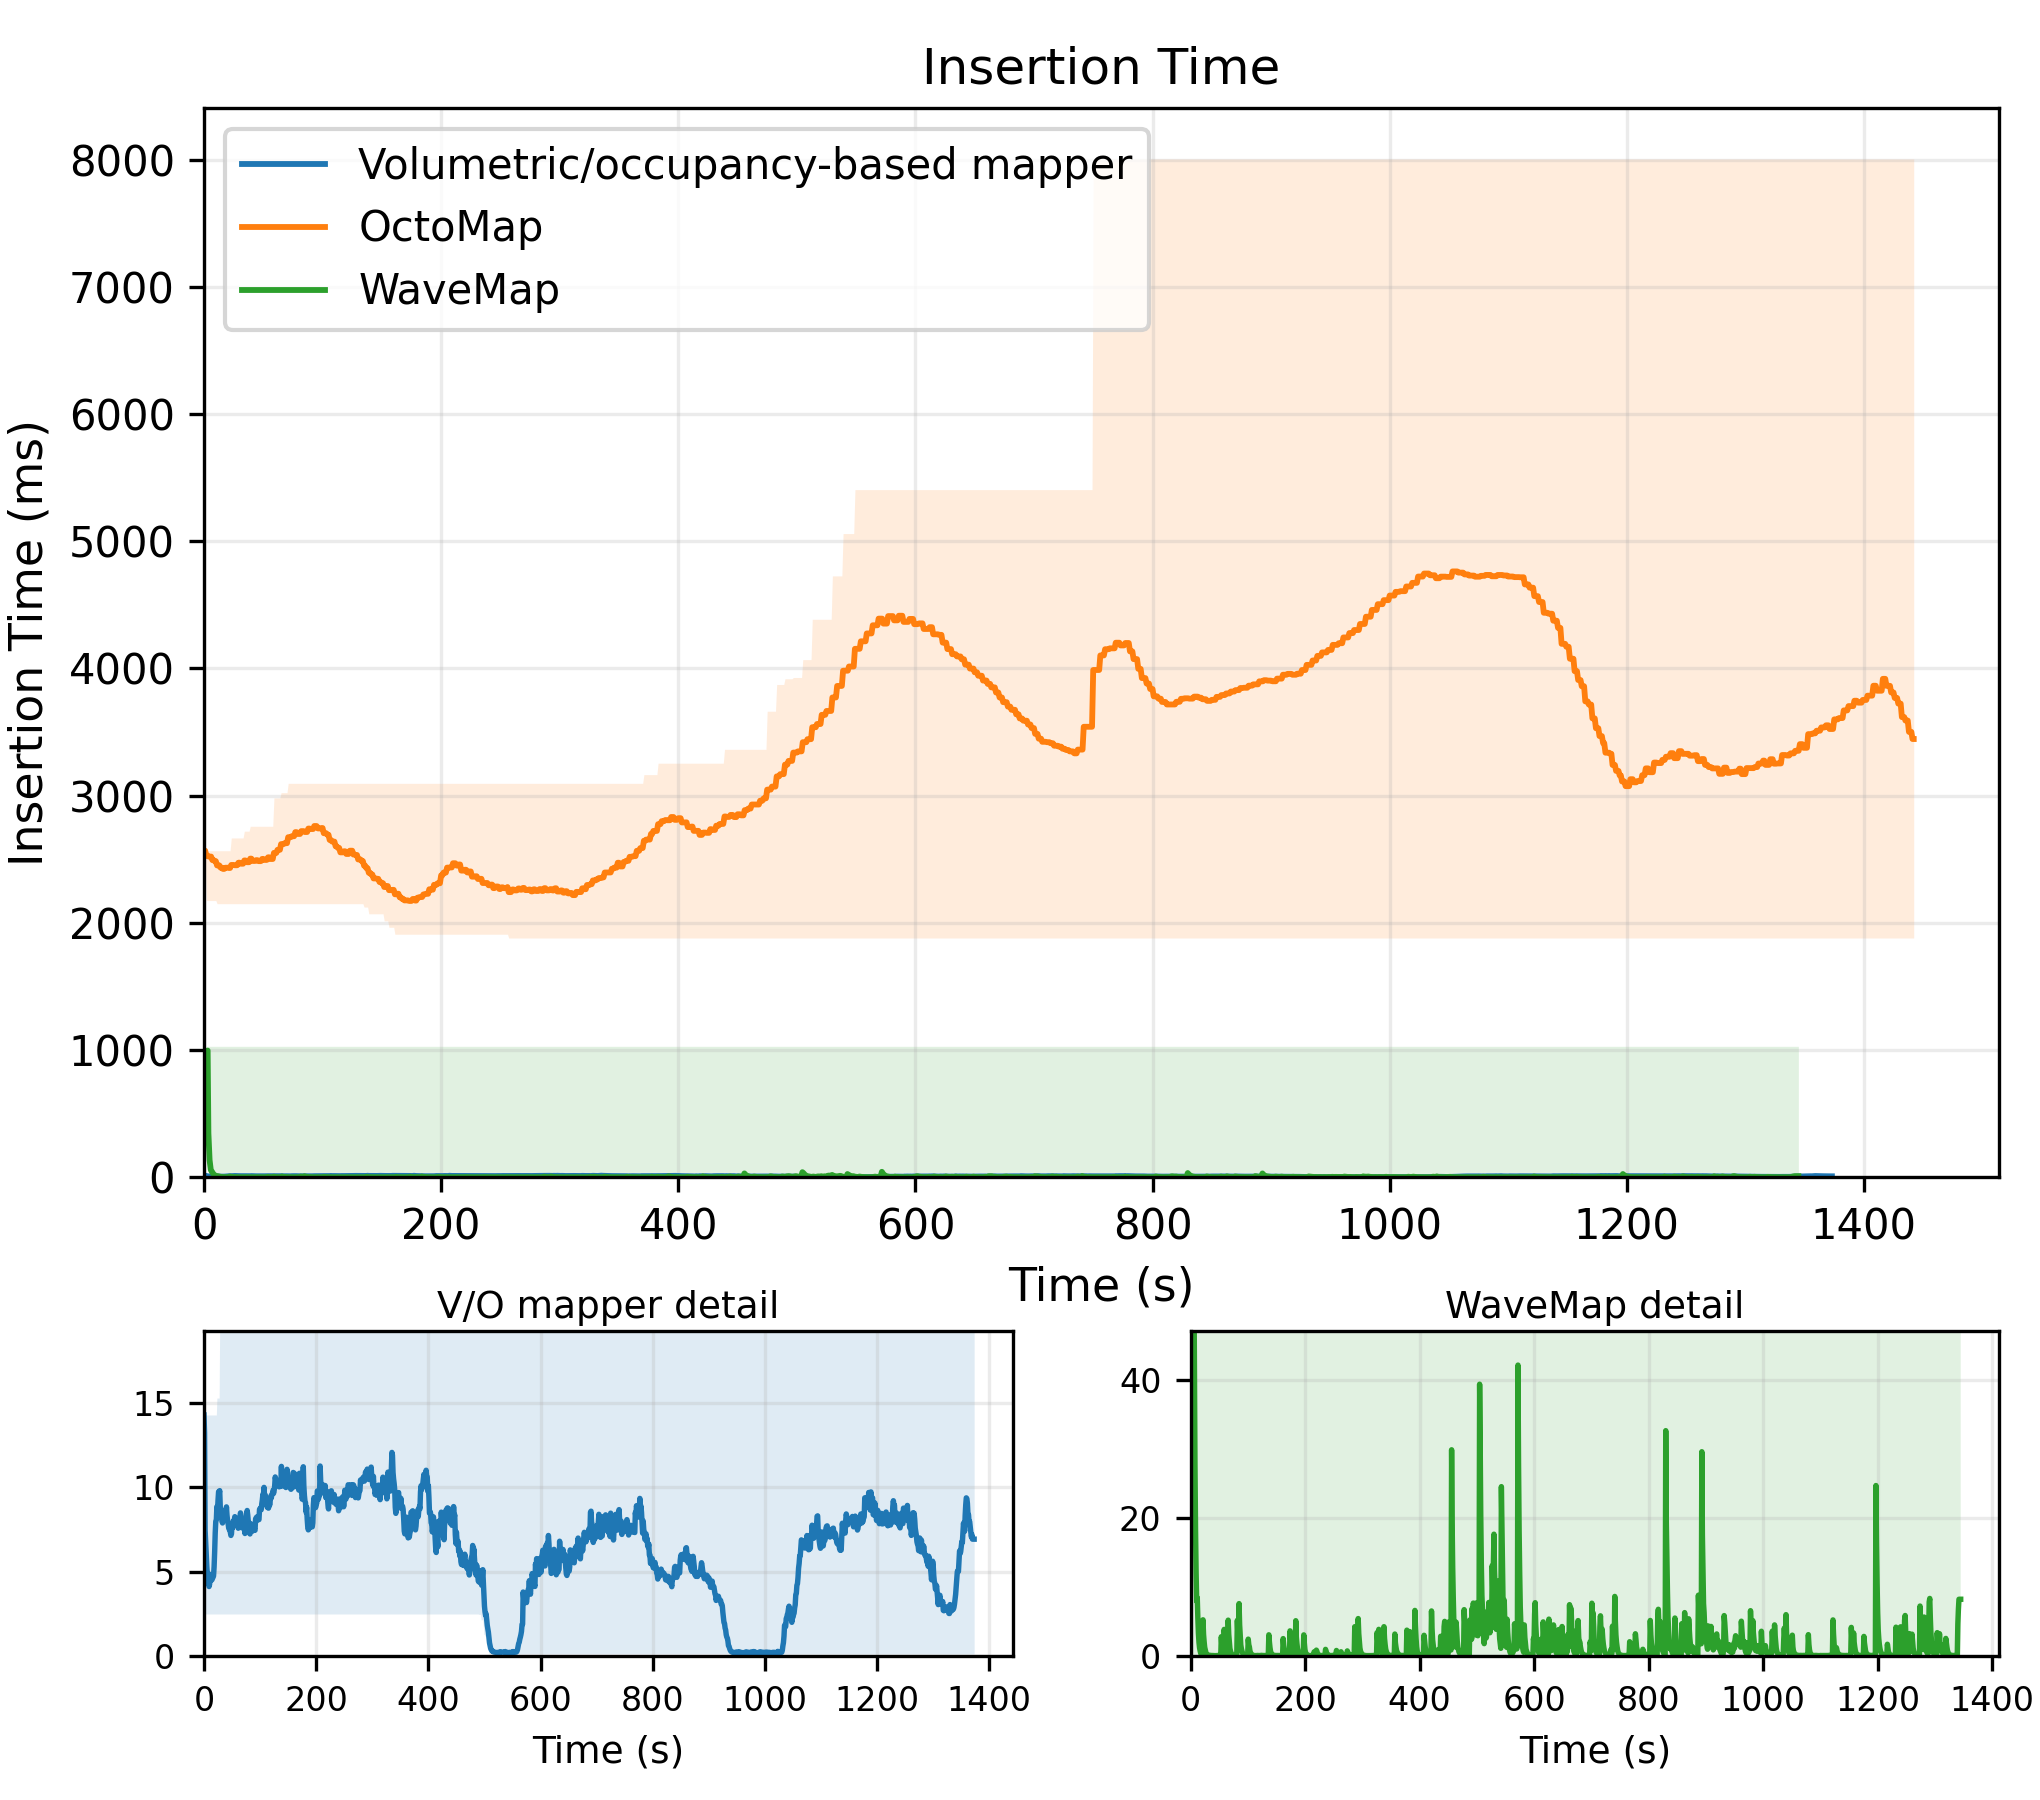
\includegraphics[keepaspectratio,height=7.5cm]{fig/plots/insertion_time.png}
	\end{figure}
\end{column}

\end{columns}

\end{frame}

\begin{frame}[t]
\frametitle{Performance Metrics}	

\vspace*{1.5cm}
\noindent
\begin{minipage}[t]{0.49\textwidth}%
	\centering
	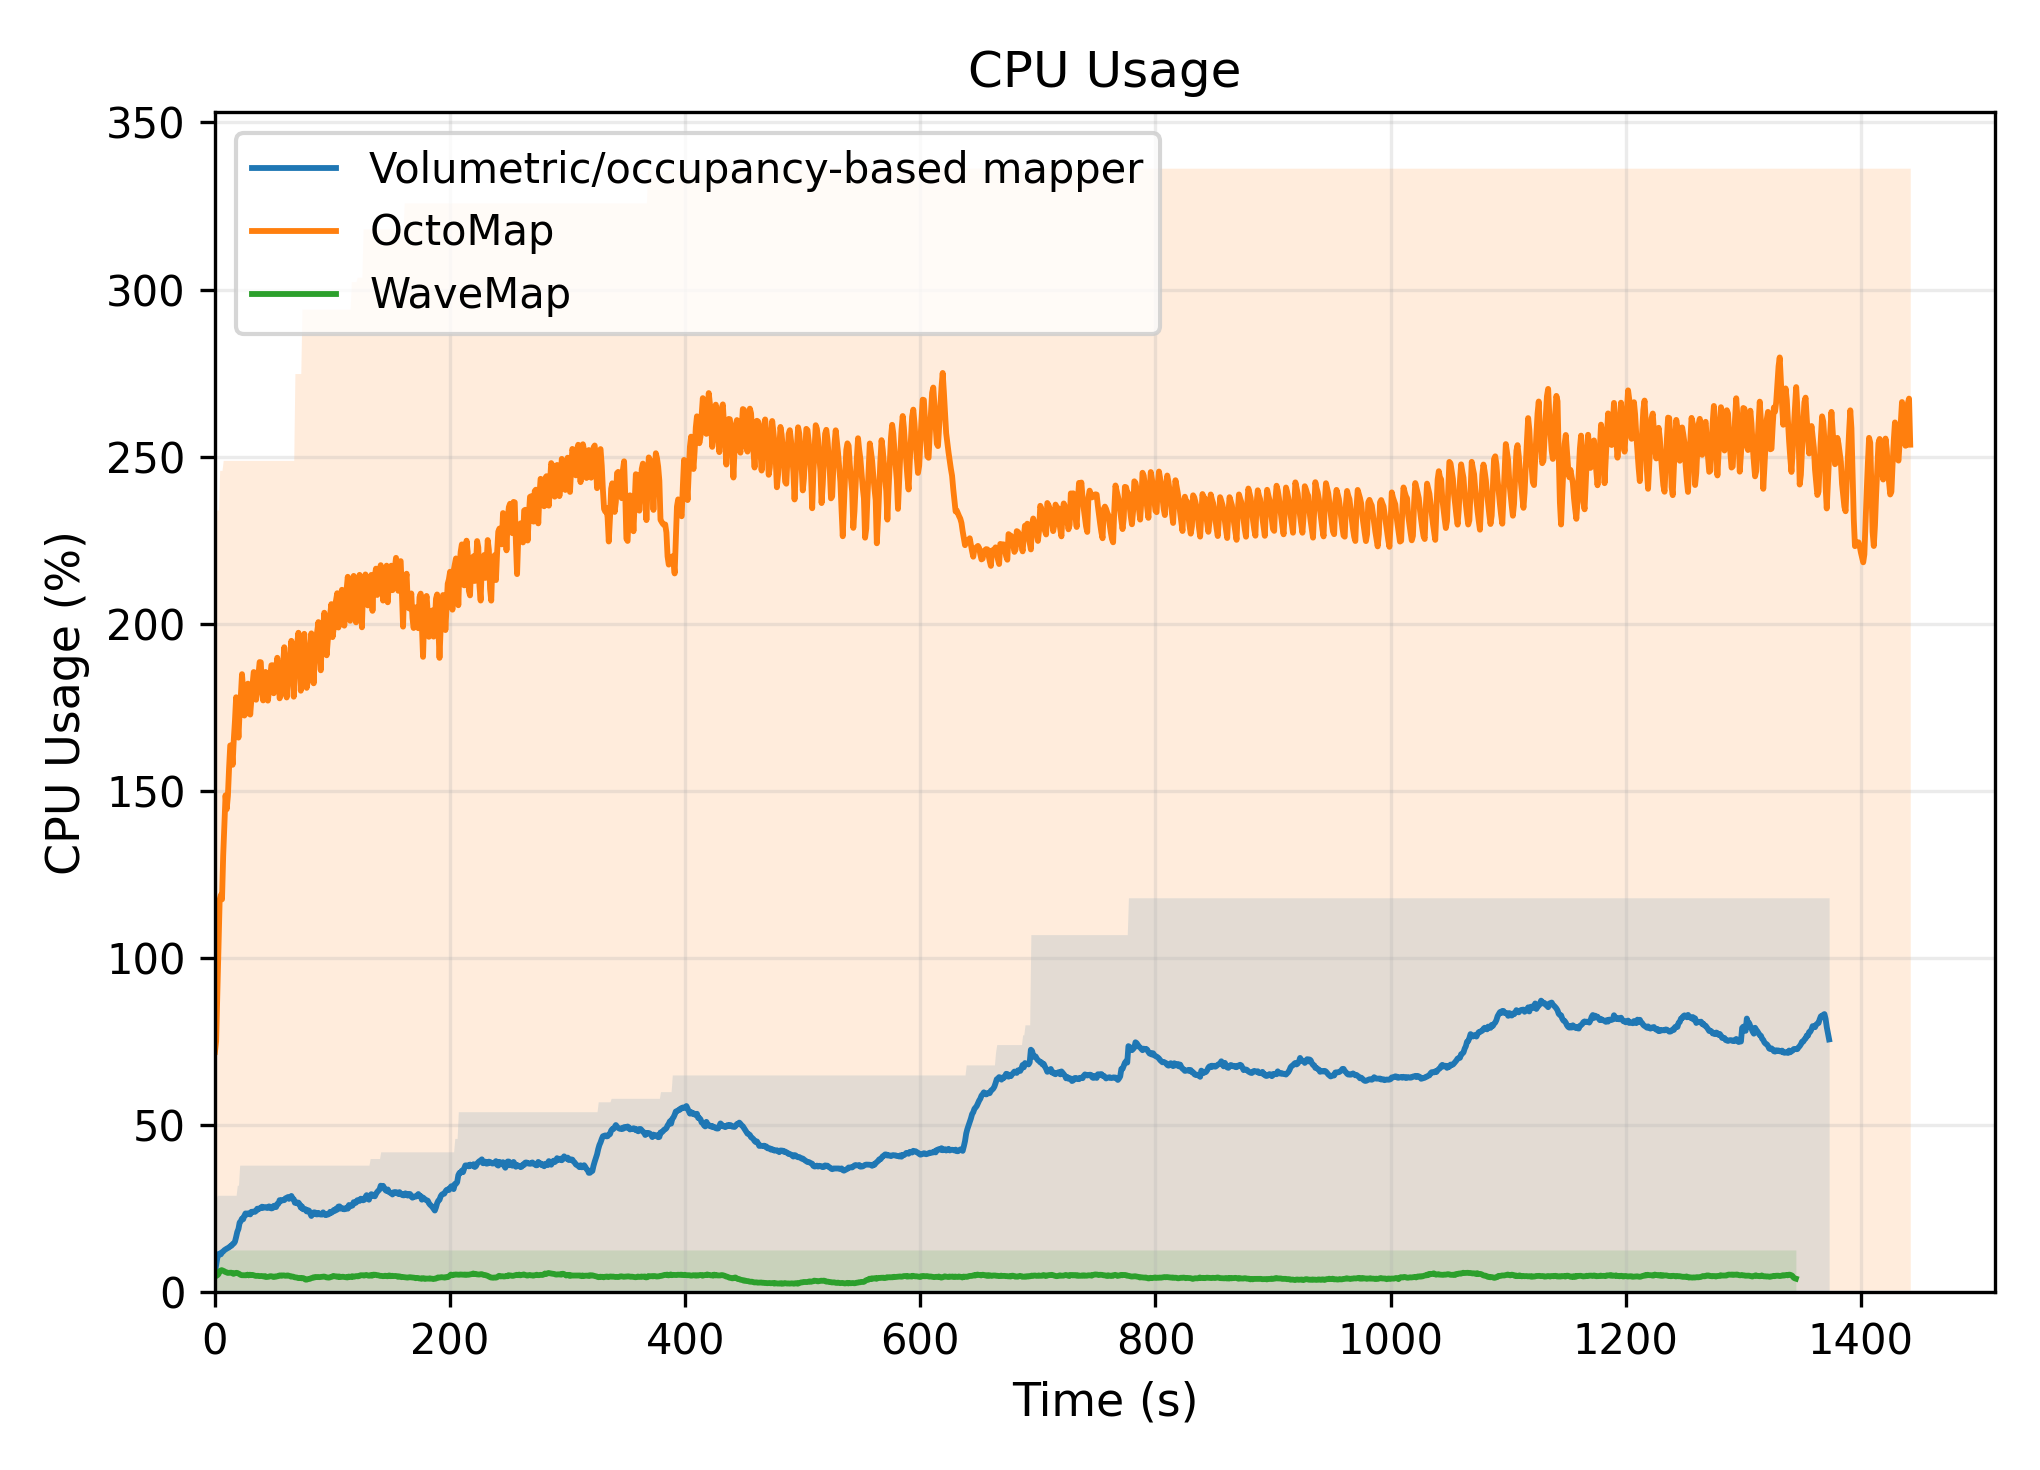
\includegraphics[
	width=\linewidth,
	height=0.8\textheight,
	keepaspectratio
	]{fig/plots/cpu_usage.png}%
\end{minipage}%
\hspace{0.005\textwidth}%
\begin{minipage}[t]{0.49\textwidth}%
	\centering
	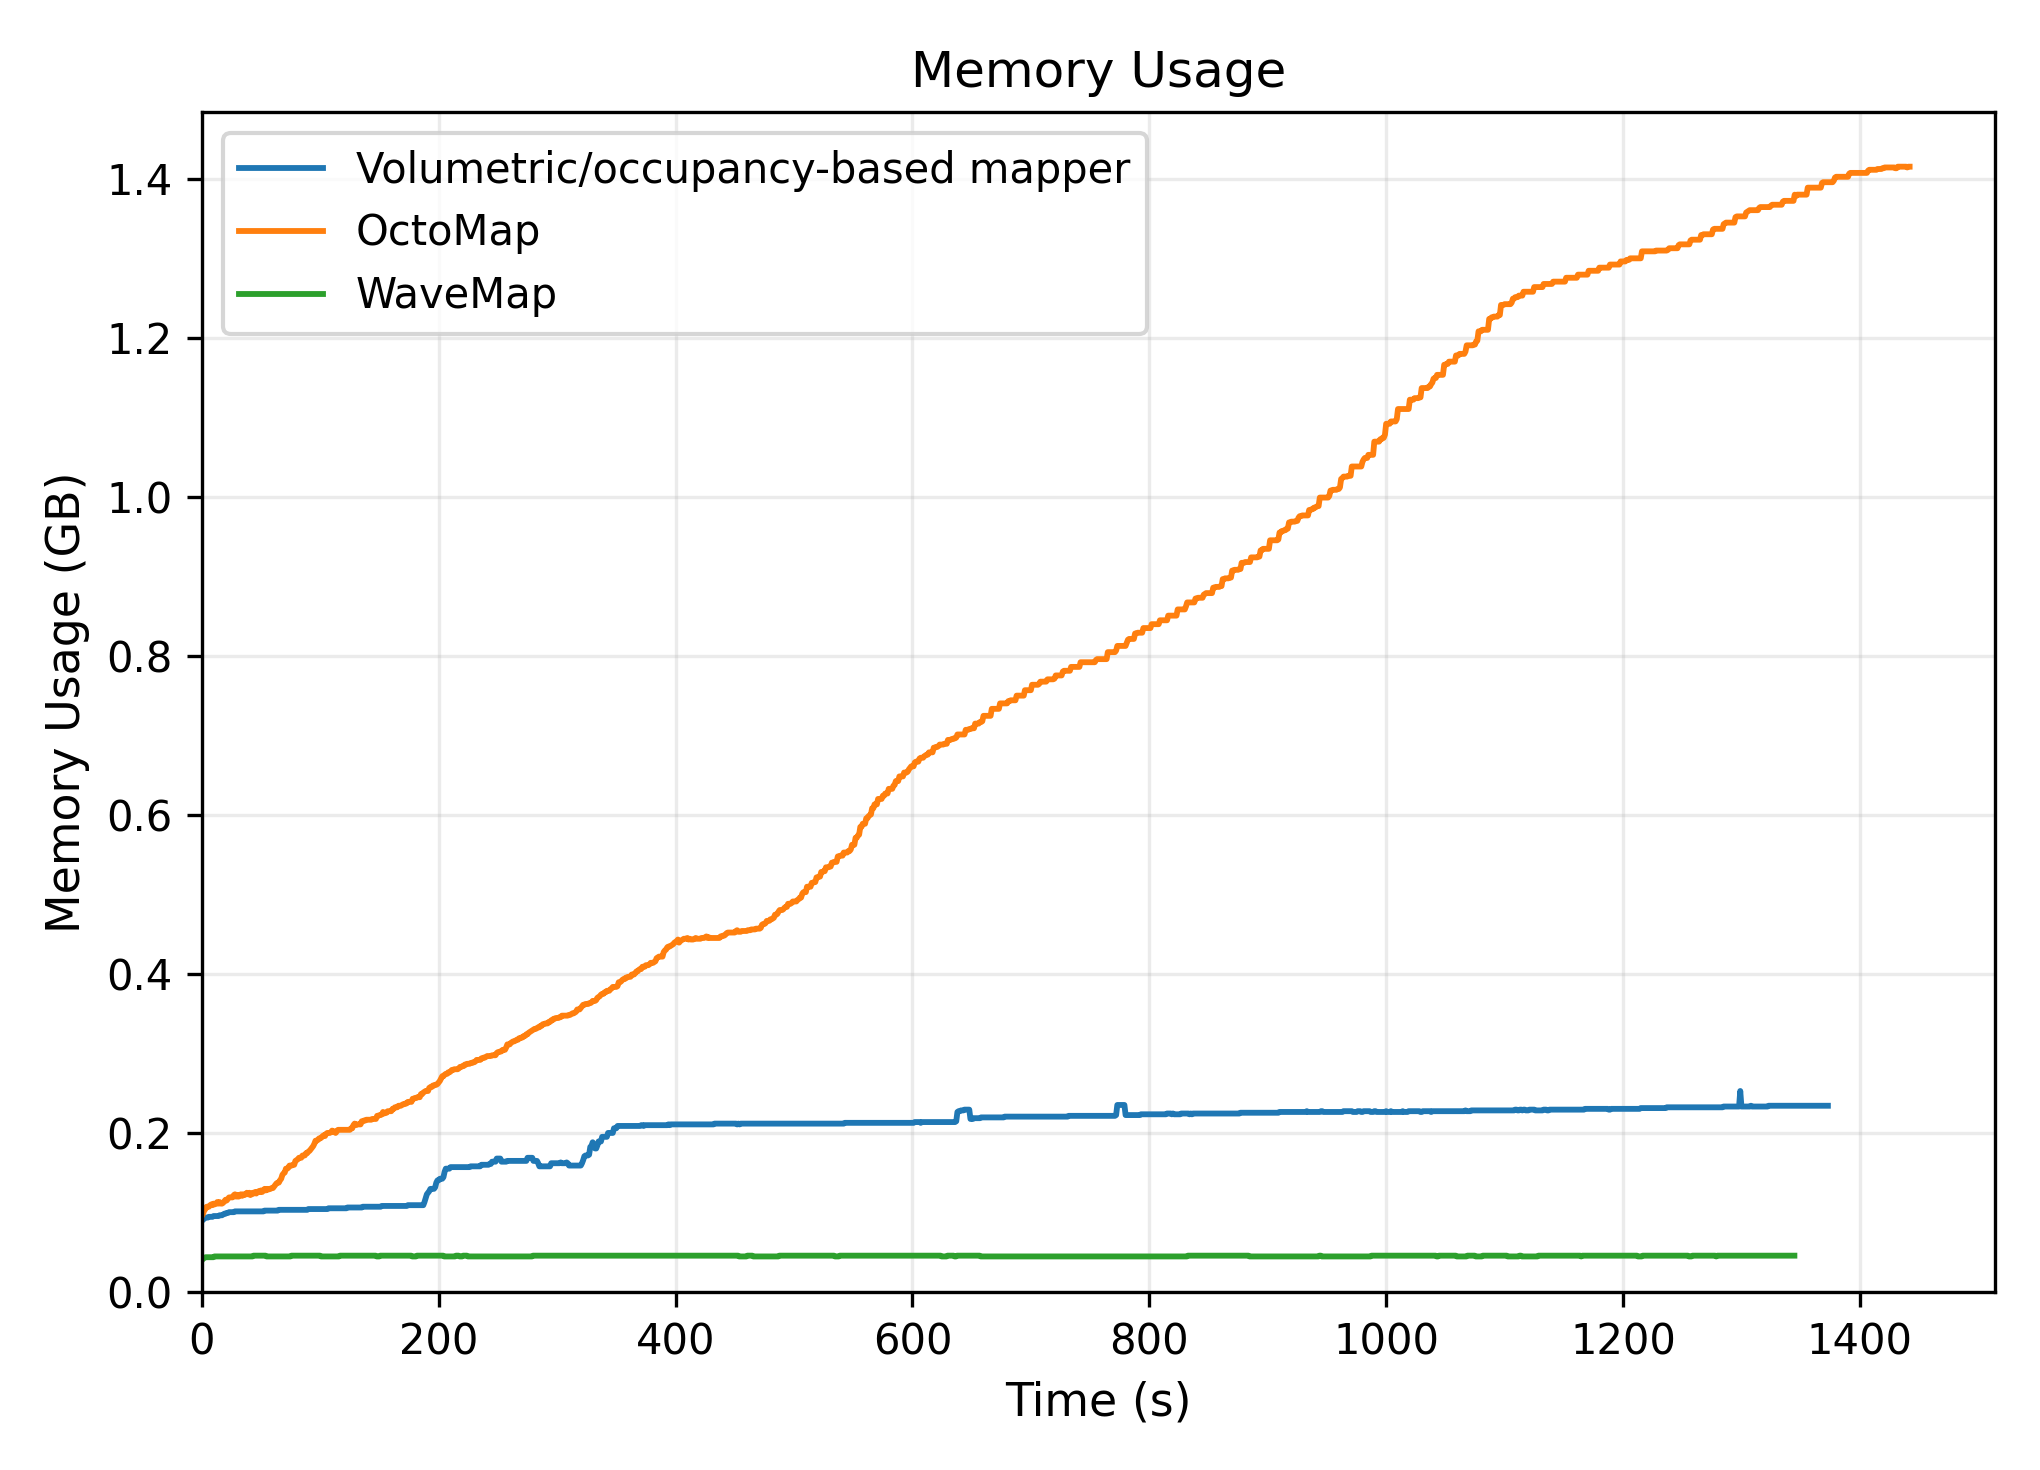
\includegraphics[
	width=\linewidth,
	height=0.8\textheight,
	keepaspectratio
	]{fig/plots/memory_usage.png}%
\end{minipage}%


\end{frame}

\begin{frame}
\frametitle{Thank You}	
	
\end{frame}

%\begin{frame}
%\frametitle{Questions}	

%\begin{center}
%	\text{TODO}
%\end{center}
	
%\end{frame}



\end{document}
